\chapter{Sistema de conversión coma flotante a coma fija y normalización }
\label{ch:Normalizacion}

El circuito implementado para la linealización se basa en el formato IEEE 754, sin embargo el estimador de parámetros, esta basado en un formato de coma fija. Se debe considerar una conversión entre ambos formatos, para esto se estudió cómo pasar de coma flotante a coma fija, ambos en 32-bits.


\section{Diseño del sistema de conversión, normalización y control}

\begin{figure}[H]
  \centering
    \includegraphics[scale=0.07]{./FF_normalizador.png}
    \rule{35em}{0.5pt}
  \caption[Diagrama general de entradas y salidas para el convertidor coma flotante a coma fija y normalizador]{Diagrama general de entradas y salidas para el convertidor coma flotante a coma fija y normalizador.}
  \label{fig:FF-NORM}
\end{figure}


La figura \ref{fig:FF-NORM} contiene el bloque general de entradas y salidas para el sistema de conversión y normalización , este posee 4 entradas: CLK , F , Begin\_FF , RST\_FF y 2 salidas: ACK\_FF , RESULT.

\begin{figure}[H]
  \centering
    \includegraphics[scale=0.07]{./FMS_FF_NORMALIZADOR.png}
    \rule{35em}{0.5pt}
  \caption[Sistema de conversión, normalización y control utilizando una máquina de estados. Señales de entrada, salida, datos y control.]{Sistema de conversión, normalización y control utilizando una máquina de estados. Señales de entrada, salida, datos y control.}
  \label{fig:FMS_FF_NORM}
\end{figure}

El sistema de conversión y normalización de la figura \ref{fig:FMS_FF_NORM} cuenta con dos módulos principales: 

\begin{compactitem}

\item \nt{Convertidor-Normalizador}: Realiza todas las operaciones requeridas para la conversión del formato coma flotante-coma fija y de la normalización, este se encarga del manejo de los datos en el cálculo. 


\item \nt{Control}: Se encarga de proveer las señales de control requeridas por el convertidor-normalizador, según las condiciones que se requiera en cada estado.

\end{compactitem}

Señales de datos: 

\begin{compactitem}

\item \nt{F}: Dato de entrada en formato IEEE 754.
\item \nt{RESULT}: Dato de salida en coma fija.

\end{compactitem}

Señales de control: 

\begin{compactitem}

\item \nt{CLK}: Reloj del sistema. Ejecuta ciclos de reloj con una frecuencia preestablecida. 

\item \nt{Begin\_FF}: Se encarga de iniciar la la unidad e indica a la máquina de estados que se debe iniciar la secuencia. 

\item \nt{RST\_FF}: Restablece los valores iniciales del sistema de conversión y normalización.

\item \nt{ACK\_FF}: Indica cuando la conversión y la normalización han sido realizadas.

\end{compactitem}


 

\section{Convertidor coma flotante - coma fija y normalizador }


\begin{figure}[H]
  \centering
    \includegraphics[scale=0.08]{./conversion_FF.png}
    \rule{35em}{0.5pt}
  \caption[Diagrama general del sistema de conversión de coma flotante a coma fija y normalización corriente-tensión]{Diagrama general del sistema de conversión de coma flotante a coma fija y normalización corriente-tensión}
  \label{fig:FF}
\end{figure}



En la figura \ref{fig:FF} se puede observar el diagrama de solución, que se utilizó en el diseño de la arquitectura del convertidor-normalizador. 
Primeramente ingresa el número en formato IEEE 754 32-bits, seguidamente se efectúa la conversión a coma fija, en donde se asigna un bit de signo, 5 bits de parte entera y 26 bits para la parte fraccionaria, este dato se procesa en una etapa de normalización y se obtiene el resultado. Este valor final esta normalizado para la corriente y tensión del panel, $\ V = [0,1]$ e $\ i = [-1,1]$, para el formato coma fija solo se requiere: un bit de signo, un bit en la parte entera y 30 para la parte fraccionaria; como se muestra en la figura \ref{fig:FF}. El aumento de bits en la parte fraccionaria indica una mejor precisión en el resultado. 

  
  \begin{figure}[H]
  \centering
    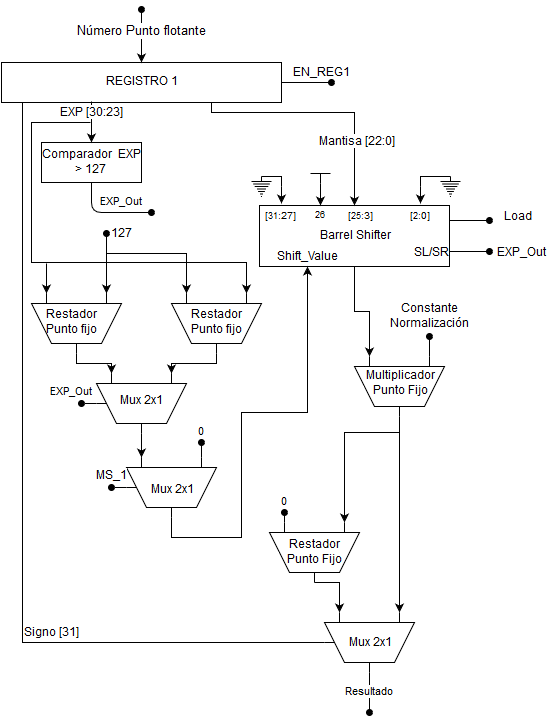
\includegraphics[scale=0.11]{./NORMALIZADOR.png}
    \rule{35em}{0.5pt}
  \caption[Circuito de conversión coma flotante a coma fija y normalización de corriente y tensión, con un dato de entrada en coma flotante y una salida en coma fija normalizada]{Circuito de conversión coma flotante a coma fija y normalización de corriente $\ [-1,1] $ y tensión $\ [0,1] $, con un dato de entrada en coma flotante y una salida en coma fija normalizada.}
  \label{fig:NORM}
\end{figure} 

Como se observa en la figura \ref{fig:NORM}, la etapa de conversión de formatos contiene un comparador, este se utiliza para saber si el número, en formato IEEE 754 contiene un exponente mayor o menor que 127. Si el número es igual a 127, indica un exponente de 0, si es mayor que 127, la bandera de salida del comparador es igual a 1 $\ \left(EXP\_Out = 1 \right)$ , si se da esta condición, se debe realizar la operación $\ EXP - 127$. Si el exponente es menor que 127, la bandera $\ EXP\_Out$  es 0 y la operación es $\ 127 - EXP$, ambas operaciones indican la cantidad de desplazamientos que se deben realizar en el desplazador de barril ("Barrel-shifter"), este se utiliza debido a que su construcción es puramente combinacional, por lo que no requiere ciclos de reloj para funcionar, esto disminuye el tiempo de cálculo en la etapa de conversión. 
La dirección de los desplazamientos se puede controlar mediante una señal que posee el desplazador de barril, esta es conectada a la bandera del comparador  $\ EXP\_Out $. El dato de entrada para el "barrel-shifter" esta compuesto por el bit mas significativo en alto (fijo) y 23 bits de la mantisa del dato de entrada en coma flotante; este dato compuesto se le aplican los desplazamientos para obtener el resultado en coma fija.    

Para normalizar un dato se requiere una división entre el máximo valor que se puede procesar, sin embargo en un circuito digital las divisiones se tornan complicadas y requieren de mucha área, por lo que se utiliza una multiplicación por una constante. Esta etapa de normalización tiene como entrada el valor convertido a coma fija, y es normalizado por medio de un multiplicador en coma fija, este requiere de una constante de normalización. 

Las constantes de normalización se pueden calcular con la siguiente ecuación: 
      

\begin{equation} \label{eq:ej1}
  C_{norm}
  = \frac{1}{Valor_{MAX}}  
\end{equation}  

La etapa de conversión y normalización se utiliza tanto para la corriente $\ i_{pv} $ como para la tensión $\ V_{pv} $ del panel, esta constante de normalización varia para cada circuito:
  
\begin{equation} \label{eq:ej2}
  Cv_{norm}
  = \frac{1}{18,1} = 0,055248618  
\end{equation}

\begin{equation} \label{eq:ej3}
  Ci_{norm}
  = \frac{1}{Ln\left(0,00667769\right)} = 0,199641045  
\end{equation}
 
 Donde $\ Cv_{norm}$ es la constante de normalización de la tensión y $\ Ci_{norm}$ la constante de normalización de la corriente. 
 
 Posteriormente a la normalización, se debe tomar en cuenta el signo del valor inicial sin convertir (coma flotante). La unidad de conversión-normalización realiza una resta $0-Dato\_coma\_fija$, y el multiplexor 2x1 del resultado selecciona el valor final en coma fija. Si el bit 32 del valor inicial es cero, el valor final en coma fija es positivo, de lo contrario el valor final en coma fija es negativo. 
  
\section{Control para el convertidor coma flotante - coma fija y normalizador}

La arquitectura diseñada para el convertidor-normalizador en su mayoría es combinacional sin embargo requiere un control, que detecta si se deben realizar desplazamientos, y cuando se debe almacenar datos en registros. 

\begin{figure}[H]
  \centering
    \includegraphics[scale=0.07]{./MaquinaFF.png}
    \rule{35em}{0.5pt}
  \caption[Sistema de control para el convetidor-normalizador, diseñado mediante una máquina de estados finita]{Sistema de control para el convetidor-normalizador, diseñado mediante una máquina de estados finita}
  \label{fig:CTRLNORM}
\end{figure} 

El control de esta arquitectura se realiza por medio de una máquina de estado finita. El funcionamiento de la maquina se describe a continuacion:  

\begin{compactitem}
\item Estado (a): Espera la señal $\ Begin\_FF$ para que la unidad de conversión-linealización sea iniciada, de manera que se ejecute un reset en los registros. 
\item Estado (b): Guarda el dato en el \nt{Registro 1}. 
\item Estado (c): Verifica la condición $\ EXP=127 $, esta determina si se deben realizar desplazamientos.
\item Estado (f): Almacena en el desplazador de barril el dato convertido. 
\item Estado (g) Almacena el resultado final en el \nt{Registro 2}. 
\item Estado (h) Indica mediante la bandera $\ ACK\_FF$ que el dato ya fue convertido y normalizado.
\end{compactitem}

\section{Sistema de conversión-normalización implementado en verilog para una placa de desarrollo nexys-4}

Este circuito se implementó por medio de el lenguaje de descripción de hardware "Verilog", realizando pequeños bloques pertenecientes a cada elemento requerido por la arquitectura diseñada. Se implementa la unidad de conversión-normalización y la unidad de control en bloques separados, de manera que se pudieran realizar pruebas sin dependencia de los bloques entre si, para una mejor depuración de errores y re-diseño>. Se realizan las simulaciones al bloque completo y se verifica su funcionamiento como se muestra en la figura \ref{fig:SIMNORM}. 

\begin{figure}[H]
  \centering
    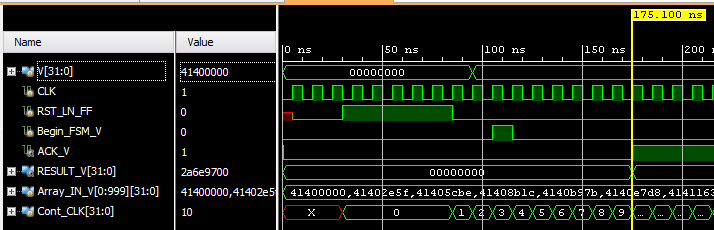
\includegraphics[scale=0.8]{./TEST_CONV_NOM_I.png}
    \rule{35em}{0.5pt}
  \caption[Simulación del circuito de conversión y normalización, ingresando en la entrada un archivo de texto, con 1000 valores de corriente lineal]{Simulación del circuito de conversión y normalización, ingresando en la entrada un archivo de texto, con 1000 valores de corriente lineal.}
  \label{fig:SIMNORM}
\end{figure}



\section{Resultados de la simulación post-síntesis del sistema de conversión-normalización}

En la implementación de un diseño en hardware, es de suma importancia simular y verificar que este funcione de manera adecuada al comportamiento esperado teóricamente. Para la comprobación de la unidad de conversión-normalización, se realizó una serie de pruebas, programando una simulación ("testbench") con mil valores de entrada, ingresados por medio de un archivo de texto previamente editado, este contiene los datos de entrada del comportamiento según el modelo del panel. 
Las pruebas de esta unidad se realizaron con valores de corriente $ i_{pv}$ y valores de tensión $ V_{pv}$, como se muestra en la tabla \ref{Table:comparacion_norm}. 

\begin{table}[H]
\centering
\caption{Comparación de resultados experimentales obtenidos por medio de una simulación post-síntesis, a partir de los valores de entrada de corriente y tensión para el circuito de conversión-normalización. CLK=100MHz }
\label{Table:comparacion_norm}
\begin{tabular}{|c|c|c|c|c|c|c|}
\hline
$  $ & Corriente  & Tensión        \\ \hline

\begin{tabular}[c]{@{}c@{}} Error máximo (\%)
\end{tabular}  & 0,0024837 & 0,0024837            \\ \hline

\begin{tabular}[c]{@{}c@{}} Error promedio (\%)
\end{tabular}  & 0,002478    & 0,002478        \\ \hline

\begin{tabular}[c]{@{}c@{}} Desviación estándar ($ x10^{-6}$)
\end{tabular} & 1,94953 & 1,94953      \\ \hline

\begin{tabular}[c]{@{}c@{}} Número de ciclos 
\end{tabular} & 8 & 8           \\ \hline

\begin{tabular}[c]{@{}c@{}} Frecuencia de ejecución (MHz) 
\end{tabular} & 12.5 & 12.5          \\ \hline

\begin{tabular}[c]{@{}l@{}} Tiempo de ejecución ($ ns$)
\end{tabular} & 80 & 80        \\ \hline

\end{tabular}
\end{table}

  \begin{figure}[H]
  \centering
    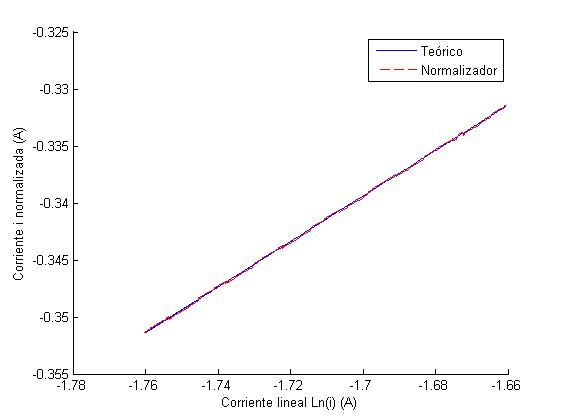
\includegraphics[scale=0.8]{./Normalizador_I.png}
    \rule{35em}{0.5pt}
  \caption[Comparación entre la conversión-normalización de corriente $\ i_{pv}$ teórica y la simulación post-síntesis del circuito]{Comparación entre la conversión-normalización de corriente $\ i_{pv}$ teórica y la simulación post-síntesis del circuito}
  \label{fig:NORMI}
\end{figure}

\newpage

En la figura \ref{fig:NORMI} se presenta la comparación entre los resultados obtenidos teóricamente y experimentalmente, a través de la simulación post-sintesis del circuito normalizador-linealizador, este toma datos de entrada con valores de corriente en formato coma flotante y retorna valores de corriente normalizados y en formato coma fija. Estos resultados se pueden comparar por medio del porcentaje de error asociado entre el valor teórico y experimental .  

  \begin{figure}[H]
  \centering
    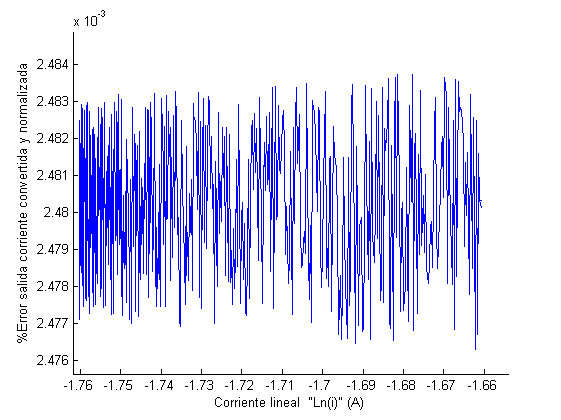
\includegraphics[scale=0.8]{./ERROR_CONV_NORM_I.png}
    \rule{35em}{0.5pt}
  \caption[Porcentaje de error entre la conversión-normalización de corriente $\ i_{pv}$ teórica y experimental del circuito]{Porcentaje de error entre la conversión-normalización de corriente $\ i_{pv}$ teórica y experimental del circuito}
  \label{fig:ENORMI}
\end{figure}

En la figura \ref{fig:ENORMI} se puede observar el error entre la conversión de la corriente normalizada teórica y experimental, con un error porcentual máximo de 0,0024837\%, un error promedio de 0,002478\% y una desviación estándar de $ 1,94953 \cdot 10^{-6} $.


  \begin{figure}[H]
  \centering
    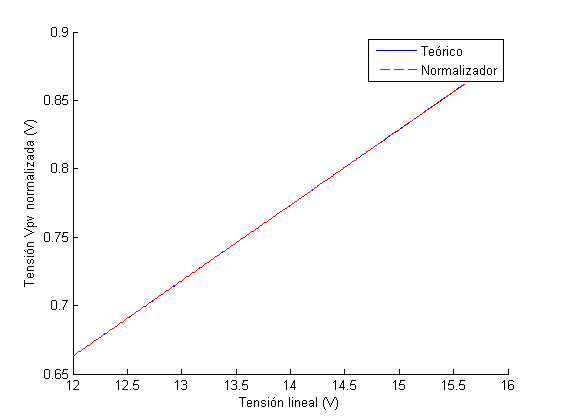
\includegraphics[scale=0.8]{./Normalizador_V.png}
    \rule{35em}{0.5pt}
  \caption[Comparación entre la conversión-normalización de tensión $\ V_{pv}$ teórica y la simulación post-síntesis del circuito]{Comparación entre la conversión-normalización de tensión  $\ V_{pv}$ teórica y la simulación post-síntesis del circuito}
  \label{fig:NORMV}
\end{figure}


  \begin{figure}[H]
  \centering
    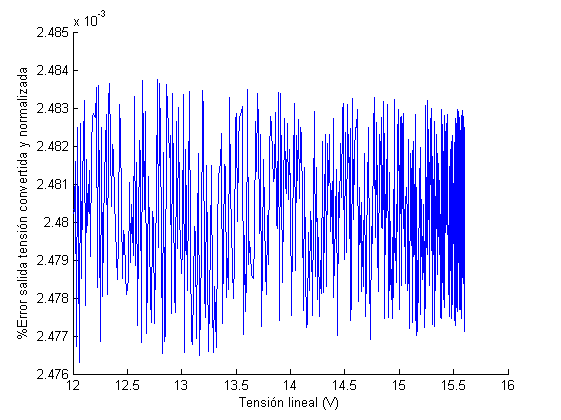
\includegraphics[scale=0.8]{./ERROR_CONV_NORM_V.png}
    \rule{35em}{0.5pt}
  \caption[Porcentaje de error entre la conversión-normalización de tensión $\ V_{pv}$ teórica y del circuito]{Porcentaje de error entre la conversión-normalización de tensión $\ V_{pv}$ teórica y del circuito}
  \label{fig:ENORMV}
\end{figure}

\newpage 

Un análisis similar al que se realizó para la conversión-normalización de la corriente, se utiliza para los resultados de la tensión. En la figura \ref{fig:NORMV} se muestran los resultados obtenidos con una tensión de entrada y su normalización, tanto teórico como experimental. Se puede calcular el porcentaje de error entre ambas curvas (teórica y experimental). En la figura \ref{fig:ENORMV} se puede observar el error con un máximo de 0,0024837\%, un error promedio de 0,002478\% y una desviación estándar de $ 1,94953 \cdot 10^{-6} $.

Esta unidad contiene muchos bloques combinacionales, por lo que se requieren pocos ciclos de reloj en la máquina de estados para realizar la conversión y la normalización. Se requieren 8 ciclos de reloj para que el resultado sea concluido, esto se puede comprobar por medio de las  simulaciones efectuadas al circuito, como se mostró en la  figura \ref{fig:SIMNORM} .
